\documentclass[a4paper,12pt]{article}
\usepackage{listing}
\usepackage{graphicx}
\begin{document}
\title{First Readers-Writers Problem}
\author{Santhisenan A}
\date{\today}
\maketitle
    
\section{Readers-Writers Problem}
In the readers-writers problem there are some processes ( termed readers ) who only read 
the shared data, and never change it, and there are other processes ( termed writers ) 
who may change the data in addition to or instead of reading it. There is no limit to how 
many readers can access the data simultaneously, but when a writer accesses the data, 
it needs exclusive access.


The first readers-writers problem gives priority to readers. In this problem, if a reader 
wants access to the data, and there is not already a writer accessing it, then access is 
granted to the reader. A solution to this problem can lead to starvation of the writers, 
as there could always be more readers coming along to access the data. 
( A steady stream of readers will jump ahead of waiting writers as long as there is currently 
already another reader accessing the data, because the writer is forced to wait until the data 
is idle, which may never happen if there are enough readers. )
\subsection{Code}
    
\begin{verbatim}
import sys

lock = 0
no_of_readers = 0

def reader():
    global no_of_readers
    print("Input: Reader")
    if lock:
        print("A wirter has acquired the lock, please wait till it releases the lock")
        return
    else:   
        no_of_readers += 1
        print("The reader can read.")

def release_reader():
    global no_of_readers    
    if(no_of_readers == 0):
        print("No readers")
    else:
        no_of_readers -= 1

def writer():
    global lock
    if lock:
        print("Another writer is reading.")
    elif no_of_readers:
        print("Another reader(s) is(are) reading")
    else:
        lock = 1
def release_writer():
    global lock
    if lock == 0:
        print("No writer is writing")
    else:
        lock = 0

while True:
    read = input()
    if read == 'read':
        reader()
    elif read == 'write':
        writer()
    elif read == 'relread': # release reader
        release_reader()
    elif read == 'relwrite': # release writer
        release_writer()
    else: 
        sys.exit()        
\end{verbatim}


\section{output}
\begin{figure}
        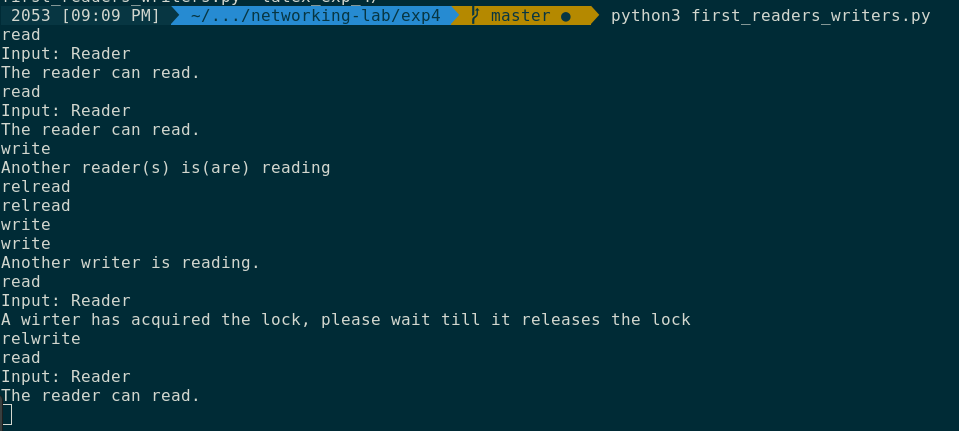
\includegraphics[width=\linewidth]{first-readers-writers.png}
        \caption{first-readers-writers}
      \end{figure}
      
       
\end{document}